\documentclass[epsfig,a4paper,11pt,titlepage,oneside,openany]{book}
\usepackage{epsfig}
\usepackage{plain}
\usepackage{setspace}
\usepackage[paperheight=29.7cm,paperwidth=21cm,outer=2cm,inner=2cm,top=2cm,bottom=2cm]{geometry}
\usepackage{titlesec} % per formato custom dei titoli dei capitoli

\usepackage{hyperref}
\usepackage{listings}

\usepackage{graphicx}
\graphicspath{ {./images/} }

\begin{document}


\pagenumbering{gobble}

% Pagina iniziale
\pagestyle{plain}

\thispagestyle{empty}

\begin{center}
  \begin{figure}[h!]
    \centerline{
\psfig{file=marchio_unitrento_colore_it_202002.eps,width=0.6\textwidth}}
  \end{figure}

  \vspace{2 cm} 

  \LARGE{Department of Information Engineering and Computer Science\\}

  \vspace{1 cm} 
  \Large{NETWORK SECURITY\\LABORATORY REPORT}

  \vspace{2 cm} 
  \vspace{1 cm} 
  \Huge\textsc{LAB 10\\HONEYPOT}


  \vspace{2 cm} 
  \begin{tabular*}{\textwidth}{ c @{\extracolsep{\fill}} c }
  \Large{Da Rold Giovanni}& \Large{Meschini Marcello}\\
  \Large{224291}& \Large{220222}\\
  \end{tabular*}

  \vspace{2 cm} 

  \Large{Academic year 2020/2021}
  
\end{center}
\clearpage

\pagestyle{plain}
\mainmatter
% indice
\tableofcontents
\clearpage
    
    
          
% gruppo per definizone di successione capitoli senza interruzione di pagina
\begingroup
% nessuna interruzione di pagina tra capitoli
% ridefinizione dei comandi di clear page
\renewcommand{\cleardoublepage}{} 
\renewcommand{\clearpage}{} 
\titleformat{\chapter}
  {\normalfont\Huge\bfseries}{\thechapter}{1em}{}
  
\titlespacing*{\chapter}{0pt}{0.59in}{0.02in}
\titlespacing*{\section}{0pt}{0.20in}{0.02in}
\titlespacing*{\subsection}{0pt}{0.10in}{0.02in}

\chapter*{Info about the lab} % senza numerazione
\label{info}

\addcontentsline{toc}{chapter}{Info about the lab} % da aggiungere comunque all'indice
\section*{Requirements}
\begin{itemize}
\item Docker Engine version 17.05 or newer
\item Docker Compose version 1.20.0 or newer
\item 2 GB of RAM
\item At least 20 GB of disk
\end{itemize}

\section*{Network Topology}
To create a network for the laboratory we used Docker Compose and created the following topology:
\begin{center}
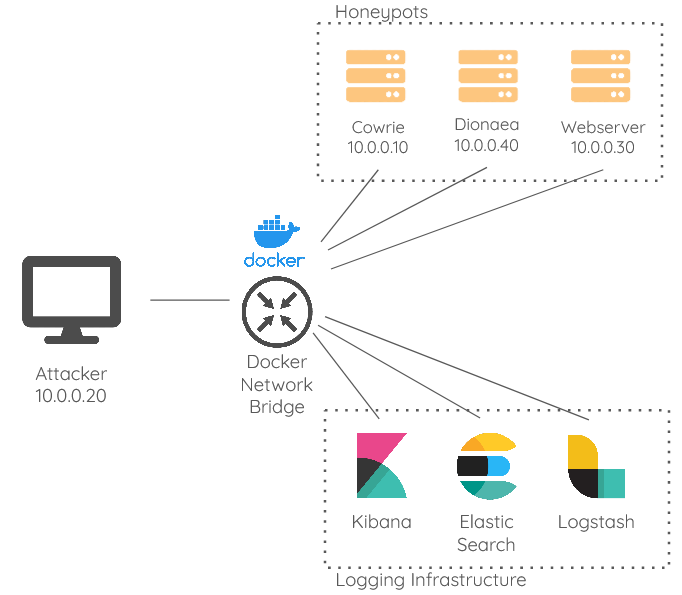
\includegraphics[scale=0.25]{topology}
\end{center}
The docker-compose.yaml file containing the definition for the containers can be found in the netsec-honeypot-lab folder on the desktop or in our Github public repository: 

\url{https://github.com/Marcy-P/netsec-honeypot-lab}

\noindent The repository README also contains additional info for accessing the containers and the references to some Docker images we used.

\section*{Starting up the lab}
To start the laboratory login into the VM with the credentials: username: \textit{netsec} and password: \textit{password}. Then open a terminal in the folder \textbackslash netsec-honeypot-lab on the desktop and type the following command:

\begin{lstlisting}[language=bash]
$ ./start.sh
\end{lstlisting}

\section*{Shutting down the lab}
To shut down the docker-compose network type:

\begin{lstlisting}[language=bash]
$ docker-compose down
\end{lstlisting}

\noindent To also clean the persistent data present in Elasticsearch type:

\begin{lstlisting}[language=bash]
$ docker-compose down -v
\end{lstlisting}

\chapter{What is a honeypot?}
\label{cha:intro}

"A honeypot is a network-attached system set up as a decoy to lure cyber attackers and detect, deflect and study hacking attempts to gain unauthorized access to information systems"\cite{techtarget}. So it is a system that is unprotected and serves no business purpose but sits in the network waiting to be contacted. Every interaction with a honeypot is suspicious because no legitimate user should utilize it.

\chapter{Characteristics of a honeypot}
\label{cha:characteristics}

Honeypots have four main characteristics; they have to be: \textbf{Deceptive} , \textbf{Discoverable}, \textbf{Interactive}, \textbf{Monitored}.

\section{Deception}

Deception can be defined as an advantageous distortion of an adversary's perceptions of reality. Honeypots heavily use this concept as a tool because they appear as real systems, but they do not serve any functional purpose for a business.

There are various frameworks that try to classify various deception strategies, and we considered the taxonomy proposed by Bell and Whaley \cite{Whaley}. According to this model deception consists in two main parts: hiding the real (dissimulation) and showing the false (simulation).

Honeypots are meant to be reachable, so you do not hide it entirely, but you often have to hide specific features of them to make them less suspicious.
The techniques to hide the real are:
\begin{itemize}
\item \textbf{Masking}: hide the  real by making relevant objects be undetectable or blend into the background;
\item \textbf{Repackaging}: hide the  real by making it appear like it is something different;
\item \textbf{Dazzling}: hide the real by altering an object to confuse the adversary;
\end{itemize}

The techniques to show the false are:
\begin{itemize}

\item \textbf{Mimicking}: show the false by using characteristics present in the actual real object;
\item \textbf{Inventing}: show the false by giving the perception that a relevant object exist while it does not; 
\item \textbf{Decoying}: show the false by misdirecting and attracting the attacker attention away from real objects.
\end{itemize}
Note that not every honeypot has to strictly follow these techniques. It is just a theoretical framework that you may want to use when creating and deploying a honeypot. 

\section{Discoverability}
Honeypots are not meant to be accessed by legitimate users but just the attacker. So when designing your honeypot you have to consider the point of view of the attacker.
In particular, you can ask yourself the following questions:
\begin{itemize}
\item Where is the attacker more likely to enter your network?
	\begin{itemize}
	\item User workstations
	\item Vulnerable services exposed to the internet
	\item Stolen VPN credentials
	\end{itemize}
\item What tool will they use to discover your asset?
\item What assets will they be interested in?
\end{itemize}

To increase discoverability, you might also place \textbf{breadcrumbs} in systems that might be compromised. They are data that will lead the attacker to your honeypot while the attacker is gathering information needed to do lateral movement in the network. An example of breadcrumbs is a clear text document containing an URL or IP of a honeypot and some credential or SSH private keys.

\section{Interactivity}

Technically a single attacker interaction is enough to produce an alert. But is better if the honeypot responds back to the attacker for two main reasons:
\begin{itemize}
\item Each interaction that attacker does with the honeypot could provide you important information. For example, if they stole some credential, you may be able to know the account that was compromised. You may be able to find out what tool they use to enter  your network
\item Make the attacker waste time. Every second that the attacker spends interacting with the honeypot is a second you can invest into finding out which systems were compromised and isolate the attacker
\end{itemize}



\section{Monitoring}

\chapter{Honeypots classification}

\chapter{Advantages of honeypots}

\chapter{Cowrie}

\chapter{Dionaea}

\chapter{Honeytokens}

\chapter{Lab monitoring infrastructure}

\chapter{Honeypots for IoT}
\endgroup


% bibliografia in formato bibtex
%
% aggiunta del capitolo nell'indice
\addcontentsline{toc}{chapter}{Bibliography}
% stile con ordinamento alfabetico in funzione degli autori
\bibliographystyle{plain}
\bibliography{biblio}
\end{document}